% ========================================================================
\documentclass[AutoFakeBold]{resume}
% ========================================================================
% ========================================================================
\usepackage{zh_CN-Adobefonts_external}
\usepackage{linespacing_fix}
\usepackage{amsmath,bm}
\usepackage{booktabs}
\usepackage{cite}
% ========================================================================
% ========================================================================
\begin{document}
% ========================================================================
% ========================================================================
\pagenumbering{gobble}
% ========================================================================
\begin{figure}[h]
    \begin{minipage}[c]{2.15cm}
        \centering
    \end{minipage}
    \hfill
    \begin{minipage}[c]{2.5cm}
        \centering
        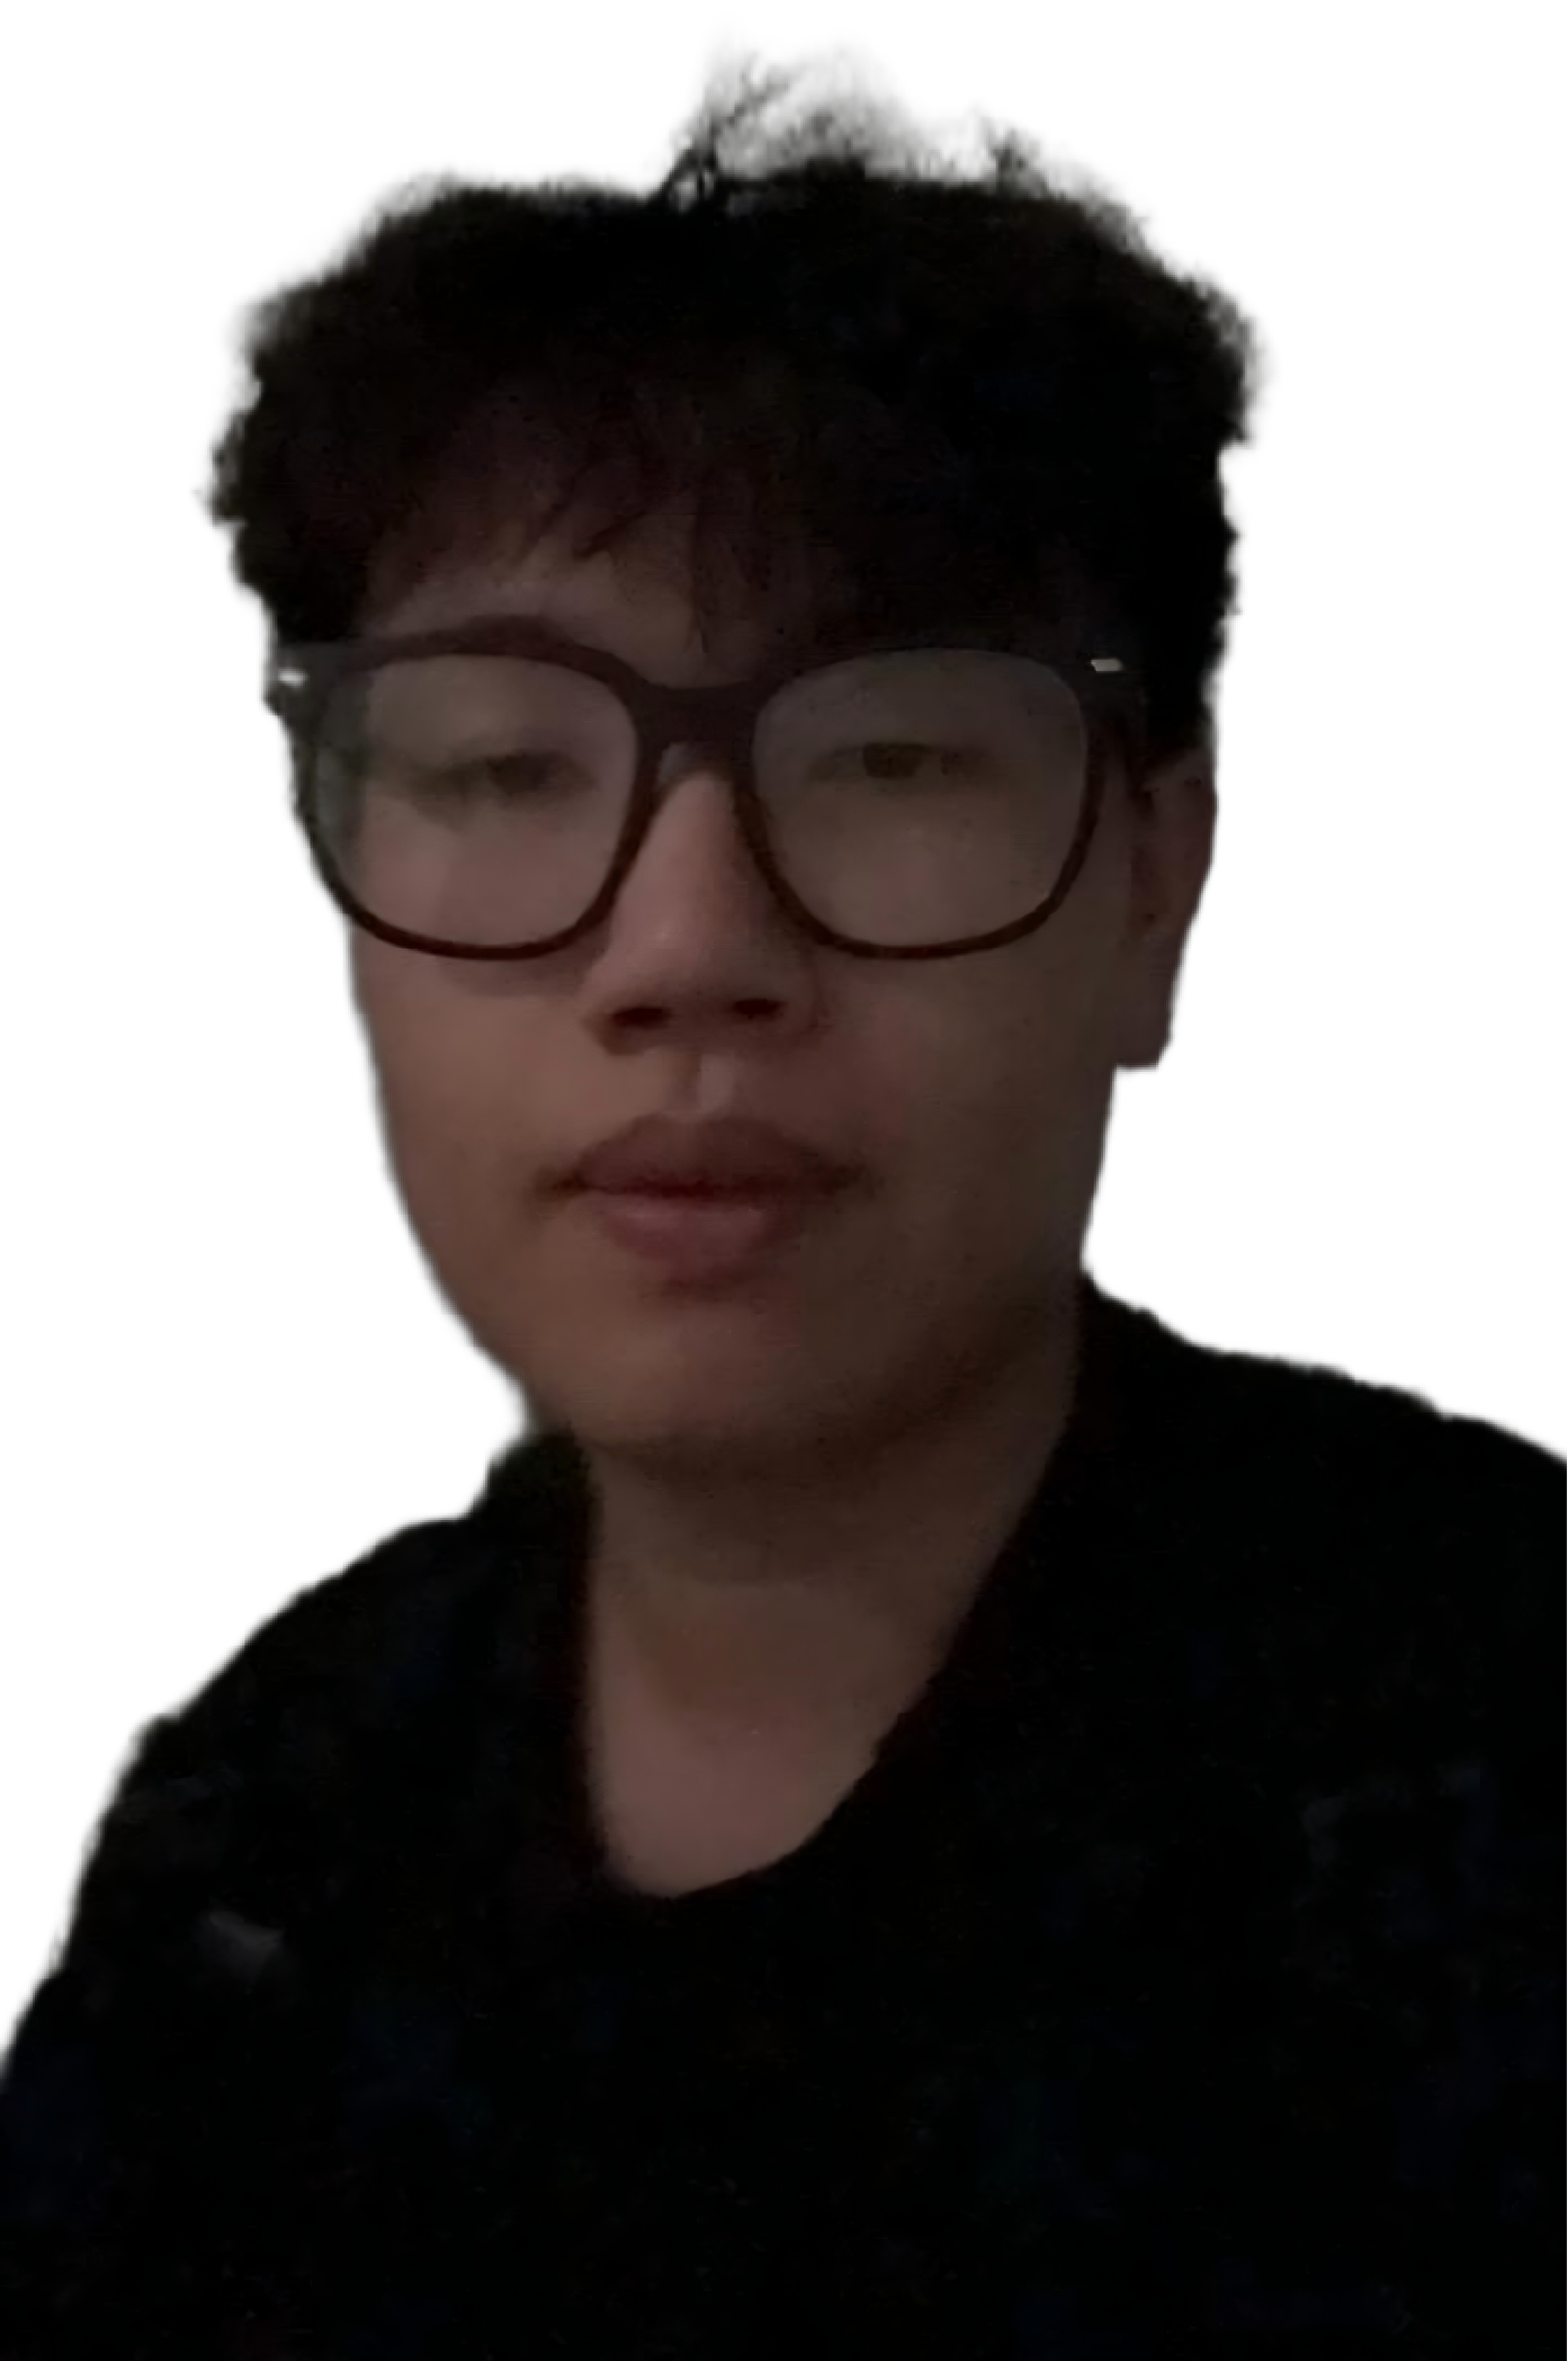
\includegraphics[height=3.2cm,width=2.4cm]{public/avatar.png}
    \end{minipage}
\end{figure}
\vspace{-32mm}
% ========================================================================
\name{\Large\textbf{\fangsong 虞瑞麒}}
% ========================================================================
\basicInfo{\faPaperPlane{中国杭州}\faCalendar{硕士研究生}}
\basicInfo{\email{richyu@hdu.edu.cn}\quad\faGithub{github.com/YRiccch}}
% ========================================================================
\vspace{.5em}
% ========================================================================
% ========================================================================
\section{\makebox[.75em][c]{\faInfoCircle} \textbf{\fangsong 基本信息}}
% ========================================================================
\vspace{1mm}
\begin{minipage}[b]{.4\textwidth}
    \centering
    \begin{itemize}
        \item[] \textbf{\kaishu 当前单位：}\kaishu 杭州电子科技大学
        \item[] \textbf{\kaishu 当前身份：}\kaishu 硕士研究生
    \end{itemize}
\end{minipage}
\hfill
\begin{minipage}[c]{.6\textwidth}
    \textbf{\kaishu 
        \begin{tabular}{ccccc}
            \toprule[1.25pt]
            专业&实验室&导师&研究方向&主页\\
            \midrule[.666pt]
            计科&VAI&周志光&可视化/HCI&YRiccch\\
            \bottomrule[1.25pt]
        \end{tabular}
    }
\end{minipage}
% ========================================================================
% ========================================================================
\section{\makebox[.75em][c]{\faGraduationCap} \textbf{\fangsong 教育背景}}
% ========================================================================
\datedsubsection{\textbf{杭州电子科技大学}\ {\faMapMarker 
\small\textbf{\fangsong 杭州}}\qquad \textbf{专业名称：计算机科学与技术}\qquad \textbf{硕士研究生}}{\textbf{2024.9 \textasciitilde \ 至今}}
\begin{itemize}
    \item \textbf{\kaishu 所属实验室: }\kaishu VAI 实验室\qquad \textbf{\kaishu 导师: }\kaishu 周志光教授
    \item \textbf{\kaishu 研究方向: }\hangindent=2em 
    \kaishu 数据可视化，人机交互，生成式 AI 与可视化的融合
\end{itemize}
% ========================================================================
\datedsubsection{\textbf{杭州电子科技大学}\ {\faMapMarker 
\small\textbf{\fangsong 杭州}}\qquad \textbf{专业名称：数字媒体技术}\qquad \textbf{本科}}{\textbf{2023.6}}
\begin{itemize}
    \item \textbf{\kaishu 学位信息: }\kaishu 获得数字媒体技术学士学位
    \item \textbf{\kaishu 相关方向: }\kaishu 数据可视化，人机交互
\end{itemize}
% ========================================================================
% ========================================================================
\section{\makebox[.75em][c]{\faPaste} \textbf{\fangsong 论文发表}}
% ========================================================================
\datedsubsection{\textbf{\textit{CompoVista: A Composition-Graph-Based Visual Analytics System for Compositional Analysis of Traditional Chinese Paintings}}}{\textbf{arXiv preprint 2026}}
\begin{itemize}
    \item \textbf{\kaishu 作者:} \kaishu Dekun Qian\textsuperscript{*}, \textbf{Ruiqi Yu\textsuperscript{*}}, Fengling Zheng\textsuperscript{\dag}, Li Ye, Yize Li, Weigui Zheng, Yigang Wang, Jinchang Li and Zhiguang Zhou\textsuperscript{\dag}
    \item \textbf{\kaishu 主题:} \kaishu 面向中国传统绘画构图分析的可视分析系统
\end{itemize}
% ========================================================================
\datedsubsection{\textbf{\textit{AniMaster: From Story Texts to Animated Videos via Cinematic Script Generation and Interactive Authoring}}}{\textbf{Manuscript, revised after ACM UIST review 2026}}
\begin{itemize}
    \item \textbf{\kaishu 作者:} \kaishu \textbf{Ruiqi Yu\textsuperscript{*}}, Dekun Qian\textsuperscript{*}, Jiale Xu, Sizhe Cheng, Yize Li, Xiangyang Wu, Zhiguang Zhou, Wei Chen and Yong Wang
    \item \textbf{\kaishu 主题:} \kaishu 从故事文本生成动画视频的脚本生成与交互式创作
\end{itemize}
% ========================================================================
\datedsubsection{\textbf{\textit{COIVis: Eye-tracking-based Visual Exploration of Concept Learning in MOOC Videos}}}{\textbf{IEEE TVCG 2026}}
\begin{itemize}
    \item \textbf{\kaishu 作者:} \kaishu Zhiguang Zhou, \textbf{Ruiqi Yu}, Yuming Ma, Hao Ni, Guojun Li, Li Ye, Xiaoying Wang, Yize Li, Yigang Wang, Yong Wang
    \item \textbf{\kaishu 主题:} \kaishu 基于眼动数据的 MOOC 视频概念学习可视探索
\end{itemize}
% ========================================================================
\datedsubsection{\textbf{\textit{HyperMOOC: Augmenting MOOC Videos with Concept-based Embedded Visualizations}}}{\textbf{ACM CHI 2026}}
\begin{itemize}
    \item \textbf{\kaishu 作者:} \kaishu Li Ye, Lei Wang, Lihong Cai, \textbf{Ruiqi Yu}, Yong Wang, Yigang Wang, Wei Chen, Zhiguang Zhou
    \item \textbf{\kaishu 主题:} \kaishu 基于概念嵌入式可视化增强 MOOC 视频学习体验
\end{itemize}
% ========================================================================
\datedsubsection{\textbf{\textit{A Hierarchical Electricity Consumption Forecasting Visualization System based on Multi-scale LSTM-KAN Model}}}{\textbf{ChinaVis 2025}}
\begin{itemize}
    \item \textbf{\kaishu 作者:} \kaishu Hang Yin, Yize Li, Ning Xu, \textbf{Ruiqi Yu}, Ningxin Li, Wei Xu, Xiangyang Wu, Jie Xu, Yongheng Wang, Zhiguang Zhou
    \item \textbf{\kaishu 主题:} \kaishu 基于多尺度 LSTM-KAN 模型的层次化电力消费预测可视化系统
\end{itemize}
% ========================================================================
\datedsubsection{\textbf{\textit{表征学习驱动的多重网络图采样}}}{\textbf{Journal of Zhejiang University SCIENCE 2022}}
\begin{itemize}
    \item \textbf{\kaishu 作者:} \kaishu \textbf{虞瑞麒}，刘玉华，沈禧龙，翟如钰，张翔，周志光
    \item \textbf{\kaishu 主题:} \kaishu 表征学习驱动的多重网络图采样方法
\end{itemize}
% ========================================================================
\section{\makebox[.75em][c]{\faTrophy} \textbf{\fangsong 访问经历}}
% ========================================================================
\vspace{.5mm}
\begin{itemize}
    \item \datedline{\kaishu 
        \begin{minipage}[t]{.45\textwidth}
            南洋理工大学计算与数据科学学院访问研究
        \end{minipage}
        \begin{minipage}[t]{.15\textwidth}
            \textbf{王勇教授}
        \end{minipage}
        }{\large\textbf{2026.03--2026.05}}
\end{itemize}
% ========================================================================
% ========================================================================
\section{\makebox[.75em][c]{\faCogs} \textbf{\fangsong 专业技能}}
% ========================================================================
\noindent
\begin{minipage}[t]{.5\textwidth}
    \begin{itemize}
    \item \textbf{\kaishu 研究方向}: 数据可视化，人机交互，生成式 AI 与可视化
    \end{itemize}
\end{minipage}
\begin{minipage}[t]{.5\textwidth}
    \begin{itemize}
    \item \textbf{\kaishu 个人兴趣}: 篮球，吉他，唱歌，旅行
    \end{itemize}
\end{minipage}
\end{document}
% ========================================================================
